    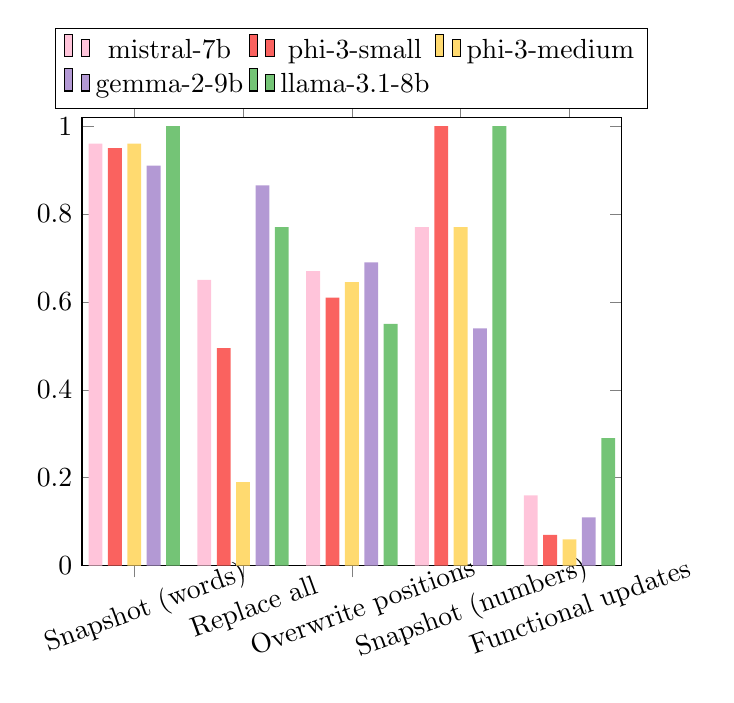
\begin{tikzpicture}
        \begin{axis}[
            ybar,
            bar width=5pt,
            symbolic x coords={Snapshot (words), Replace all, Overwrite positions, Snapshot (numbers), Functional updates},
            xtick=data,
            ymin=0, ymax=1.02,
            legend columns=3,
            legend style={at={(0.5,1.20)}, anchor=north, draw=black},
            enlarge x limits=0.12,
            xticklabel style={rotate=20, anchor=center, yshift=-12pt}
        ]
        
        \addplot[fill={rgb,255:red,255;green,196;blue,218}, draw=none] coordinates {(Snapshot (words),0.96) (Replace all,0.65) (Overwrite positions,0.67) (Snapshot (numbers),0.77) (Functional updates,0.16)};
        \addlegendentry{mistral-7b}
        
        \addplot[fill={rgb,255:red,250;green,98;blue,95}, draw=none] coordinates {(Snapshot (words),0.95) (Replace all,0.495) (Overwrite positions,0.61) (Snapshot (numbers),1.00) (Functional updates,0.07)};
        \addlegendentry{phi-3-small}
        
        \addplot[fill={rgb,255:red,255;green,218;blue,112}, draw=none] coordinates {(Snapshot (words),0.96) (Replace all,0.19) (Overwrite positions,0.645) (Snapshot (numbers),0.77) (Functional updates,0.06)};
        \addlegendentry{phi-3-medium}
        
        \addplot[fill={rgb,255:red,179;green,153;blue,212}, draw=none] coordinates {(Snapshot (words),0.91) (Replace all,0.865) (Overwrite positions,0.69) (Snapshot (numbers),0.54) (Functional updates,0.11)};
        \addlegendentry{gemma-2-9b}
        
        \addplot[fill={rgb,255:red,116;green,196;blue,118}, draw=none] coordinates {(Snapshot (words),1.00) (Replace all,0.77) (Overwrite positions,0.55) (Snapshot (numbers),1.00) (Functional updates,0.29)};
        \addlegendentry{llama-3.1-8b}
        
        \end{axis}
\end{tikzpicture}